\documentclass[output=paper]{LSP/langsci} 
\ChapterDOI{10.5281/zenodo.1090954}

\author{Michael Carl\affiliation{Renmin University of China}\lastand
Moritz Schaeffer\affiliation{Johannes Gutenberg University of Mainz}} 

\title{Sketch of a Noisy Channel Model for the translation process}

\abstract{To advance the state of the art in translation process research, \citet{Toury2004} requests the formulation of ``probabilistic explanations in translation studies''. This chapter develops these ``conditioned statements'' into a Noisy Channel Model of the translation process with the ultimate aim to predict ``particular \textit{modes of behavior}'' by their observable traces in the user activity data (UAD). We first develop a Noisy Channel Model for the translation process and then present a number of research results that may serve as a basis for the formulation of observable behavioral units and of the latent states in a noisy translation process model. However, a large amount of research has still to be conducted before we might be able to get a complete picture of the various shades and complexities of the translation process.}


\begin{document}         
\maketitle   

\section{Introduction}
\label{carl-schaeffer:sec:1}
The Noisy Channel Model \citep{Shannon1949} has been very productive for solving non-deterministic problems in communication and computational linguistics. It is a mathematical formalization of communicative processes that underlies, among many other things, speech recognition \citep{Xuedong1990}, statistical \isi{machine translation} \citep{Brown1993} and the translation of a text from a \isi{source language} to a \isi{target language}. Statistical \isi{machine translation} (SMT) models translation as a process in which a source text is decoded, thereby eliminating the \isi{noise} (e.g. adjusting lexical and syntactic divergences) to uncover the intended message (i.e. the translation). In automatic speech recognition, the speech signal is segmented, analysed and mapped onto a sequence of phones, which represents possible pronunciations of the words to be recognized.

In this chapter we develop a framework of the Noisy Channel Model for the \isi{translation process}. In analogy with speech recognition, the translation \textit{process} is modeled as a probabilistic sequence of behavioral observations, such as keystrokes and eye movements, which are emitted by underlying hidden processes. The aim of the noisy channel is to anticipate and generate the behavioral user activity  data (UAD) and to
uncover and understand the underlying hidden translation processes that are involved in the generation of the translation. 

Just as for automatic speech recognition, the segmentation and quantification of the stream of events is a precursor also for decoding translation processes. A considerable amount of work has been invested in translation \isi{process research} to define and investigate various kinds of units, measures and metrics that are suited to structure and quantify processing activities. 

On the one hand, the final outcome of the \isi{translation process} is a text (i.e. the translation) which is defined by the spatial/sequential order of the linguistic items that it constitutes. We may thus approach the \isi{translation process} from a textual angle and investigate behavioral patterns that are involved in the production of particular words or phrases. Consequently, we will deal with text-based units of investigation, spatial areas of interest (AOIs\footnote{This term was coined as a tool for the investigation of eyetracking data. It can be equally used to denote a textual area to accumulate different kinds of UAD.}) which accumulate related behavioral UAD. 

On the other hand, the translation processes can be considered a temporal sequence of translational events, which may be segmented into coherent chunks or behavioral units. For instance, \isi{pauses} in the translation production process (i.e. gaps in the typing activities) have been associated with cognitive meta-activity and pause analysis has been proposed as a method to detect the amount of '\isi{cognitive effort}' in translation (e.g. \citealt{Immonen2006, Obrien2006, Lacruz2012}). However, it is unclear what exactly the cognitive processes are that take place during typing \isi{pauses} and it is an unsolved problem to determine what exactly makes \isi{pauses} more or less effortful. In addition, recording of gaze data is required to `fill' the typing \isi{pauses} and to identify the specific motivation of a particular pause \citep[47]{Kumpulainen2015}. 

In both cases, a distinction can be made between early, automatised translation processes and later more time-consuming processes. A number of measures exist that are suited to describe early translation processes; these include fluent typing activities and early \isi{eye movement} measures such as \isi{first fixation} durations. However, late translation processes are more complex, more difficult to describe and their traces in the process data are more varied and difficult to classify or identify than the early processes.

As suggested by \citet{Toury2004}, translation processes and behavioral observations are probabilistic in nature. In this chapter, we suggest a probabilistic framework to assess and integrate several findings from empirical translation \isi{process research}. We first lay out the general ideas of the Noisy Channel Model in \sectref{carl-schaeffer:sec:2} and apply the introduced notions to the translation \isi{process research} (TPR) terminology. We show that the Noisy Channel Model provides a powerful framework to formalize ``probabilistic explanations in translation studies'' \citep{Toury2004}. 

One of the essential requirements for a noisy \isi{translation process model} is the fragmentation and quantification of the stream of UAD  into meaningful segments. \sectref{carl-schaeffer:sec:3} discusses a number of attempts to segment the UAD into meanigful units, including production units, attention units and activity units. In the \isi{noisy channel model}, these behavioral units are generated by underlying hidden translation states. Drawing on the \isi{monitor model}, we make a distinction between early and later translation processes and argue that they represent different mental states. \sectref{carl-schaeffer:sec:4} provides a number of properties for these earlier and later translation states, the output of which can be measured in the behavioral UAD.

\section{The noisy channel model in translation} 
\label{carl-schaeffer:sec:2}
The Noisy Channel Model conceptualizes communication as a problem of decoding \citep{Shannon1949}, in which a transmitter sends a message $m$ through a noisy communication channel. The receiver perceives a signal $o$ as a noisy encoded version of the original message. In order to reconstruct the message $m$, the Noisy Channel Model assumes two factors: a language model $P(m)$ which indicates the probability of the original message $m$ and the conditional probability $P(o|m)$ which quantifies the probability of the signal $o$ provided we know the message $m$. The probability $P(o|m)$ accounts for the \isi{noise} that is added during the communication process. This component analysis can be achieved with the help of Bayes' theorem, which states that a conditional probability $P(m|o)$ can be decomposed as $P(m|o) = P(o|m)*P(m)/P(o)$. Decoding makes use of the right side of this equation, ignoring the common denominator $P(o)$. The \isi{noisy channel model} is used to formalize a variety of different communication problems; in automatic speech recognition, $o$ is an acoustic signal and $m$ is the spoken message \citep{Mylonakis2007}. The model is also used for part-of-speech tagging, in syntactical analyses, and in many other natural language processing (NLP) applications. 

\begin{figure}
\begin{center}
\resizebox{\textwidth}{!}{
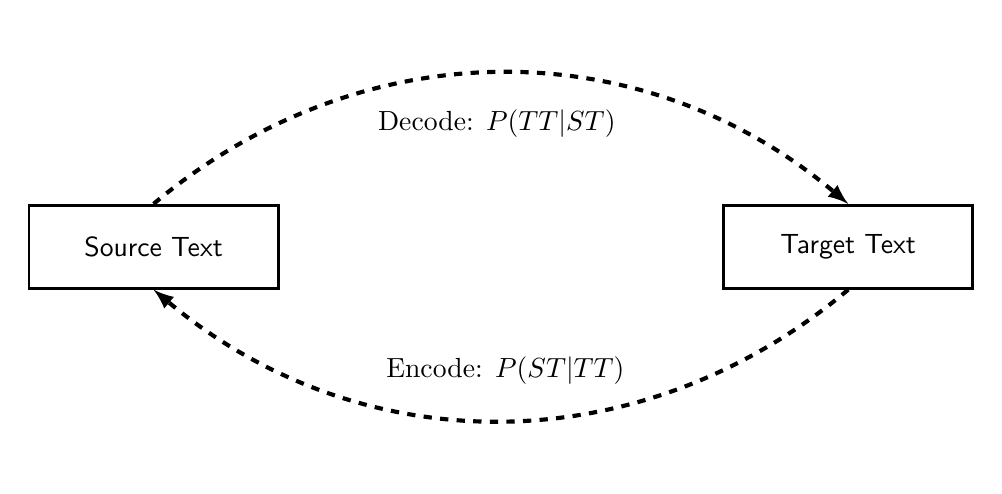
\begin{tikzpicture}
        \usetikzlibrary{shapes,arrows,positioning}
    % Define Styles
        \tikzstyle{block} = [rectangle, draw, fill=white, text centered, minimum height=3em, minimum width = 9em, line width = 0.1em]
        \tikzstyle{line} = [draw, -latex, line width=0.15em, dashed]
    % Place nodes
        \node [block] (source) {\sffamily{Source Text}};
        \node [block, right = 16em of source] (target) {\sffamily{Target Text}};
    % Draw edges
        \path [line] (source.north) to[out=40,in=140] (target.north) node [above left = 2em and 8em] {Decode: $P(TT|ST)$};
        \path [line] (target.south) to[out=-140,in=-40] (source.south) node [below right = 2em and 8em] {Encode: $P(ST|TT)$};
\end{tikzpicture}
}
%\includegraphics[width=3in]{figures/carl-schaefer/sketch-img001.png}
\end{center}

\caption{The noisy channel model for translation}
\label{carl-schaeffer:fig:ncm}

\end{figure}


In the context of SMT it is assumed that the target text (TT) corresponds to the message $m$ and the source text (ST) is the signal $o$ that we want to decode (see \figref{carl-schaeffer:fig:ncm}). Given we know all the factors that are involved in the encoding process in $P(ST | TT)$ and we know the probabilities with which each single event occurs, we can reverse the encoding process based on Bayes' law as shown in equation \ref{carl-schaeffer:eqn:bayeslaw}. 

\begin{eqnarray} 
\label{carl-schaeffer:eqn:bayeslaw}
 P(TT|ST)  & =  &  P(ST|TT) * \frac{P(TT)}{P(ST)}
\end{eqnarray}

As each of the factors that contributes to a translation (i.e. the encoding and decoding) generates a large number of hypotheses, the Noisy Channel Model makes use of a search operator $argmax$ to retrieve the most probable translation among the many possible options. 

\begin{eqnarray} 
\label{carl-schaeffer:eqn:maxprob}
\widehat {TT}  & = & argmax~~P(TT |ST) * P(TT)
\end{eqnarray}

The $argmax$ operator in equation \ref{carl-schaeffer:eqn:maxprob} takes account of the fact that there can be many possible outcomes, but we are searching only for the most likely translation  $\widehat {TT}$. This operator produces, under optimum circumstances, the best reconstruction of the translation  $\widehat{TT}$ based on observed source text (or sentence) ST.

\begin{eqnarray} 
\label{carl-schaeffer:eqn:totalprob}
P(ST|TT)  & = & \sum_i P(ST|TT, v_i)
\end{eqnarray}


Equation \ref{carl-schaeffer:eqn:totalprob} demonstrates the possibility of including additional predictor variables  $v_i$ in the Noisy Channel. Since the total probability of a sample space always amounts to  $1=\sum _i v_i$ any number of additional variables can
be introduced in this manner, so as to provide additional explanatory power to the computations. 

Early approaches to SMT modelled the channel as a probabilistic translation dictionary \citep{Brown1988}. More recent SMT systems use many additional resources, such as phrase- or tree-based translation models; they encode sentences as lattices or confusion networks that enhance the noisy channel extensively. In order to integrate a large amount of features that might impact the decoding process, the Noisy Channel Model has been generalized as shown in equation \ref{carl-schaeffer:eqn:loglin}, which can take into account any number of feature functions $f_k(ST, TT,v_k)$, which are weighted by a factor  $\lambda _k$ \citep{Och2003}. Each feature function  $f_k(\cdot)$ may represent a very different aspect in the decoding process and can be trained independent of other features. Its contribution to the overall outcome of the decoding process is ranked by a factor  $\lambda _k$:

\begin{eqnarray}
\label{carl-schaeffer:eqn:loglin}
\widehat {TT} & = & argmax~~P(TT|ST) \approx \sum_{k=1 \ldots n} \lambda_k * f_k(ST, TT,v_k) 
\end{eqnarray}

We propose an adaptation of the Noisy Channel Model to model human translation and post-\isi{editing} processes. 

\subsection{Probabilistic translation processes}
\label{carl-schaeffer:sec:2.1}

In an attempt to define the notion of translation \isi{universals}, \citet{Toury2004} requests the formulation of conditioned statements which would provide ``probabilistic explanations in translation studies''. Conditioned statements would predict ``particular \textit{modes of behavior }(or their observable results) {\dots} [based on] an array of \textit{variables}, whose capacity to enhance (or reduce) the adoption or avoidance of a particular behavior would be verified empirically'' \citep[24]{Toury2004}. The most general format of such a conditioned statement according to Toury would be as follows:

\begin{quote}
If 1 and 2, and 3, and {\dots} ${\infty}$, then there is great likelihood that X [\dots]
where the numbers (1, 2, 3, {\dots} ${\infty}$) stand for the different variables which may have an effect on the selection of a translational behavior. (p. 26)
\end{quote}

In terms of the notion introduced above, Toury's conditioned translation statement can thus equivalently be expressed as a set of conditional probabilities in the form  $P(x_i | v_1,v_2,{\dots},v_m)$ where $x_i$ stands for a particular predicted translation behavior and the set $V = \{v_1,v_2,...,v_m\}$ contains predictor variables which have an effect on and explain --- to a certain extent --- the observed behaviour $x_i$ in a probabilistic manner. Even though there might be many different modes of translation, we assume that the \isi{translation process} consists of a finite inventory of behavioral patterns $X = \{x_1,...,x_n\}$ and we assume --- in contrast to Toury --- that for each of the observations $x_i,1{\leq}i{\leq}n$ there exists only a finite set of predictor variables  $v_j \in V$ that has an effect on  $x_i$. The observed \isi{translation process}  $X$ can then be formalized as a sequence of possible behavioral patterns $x_1, x_2 \dots$ that are conditioned by a number of predictor variables $v_1, v_2 \dots$. The most likely (explanation for) translation behaviour  $\widehat{X}$ can thus be computed in a similar way as the most likely translation  $\widehat{TT}$.

The general idea in this model is that the value of a dependent variable ($X$) is related to a set of independent variables ($V$) through a function ($F$). Given the translation UAD, we learn the function ($F$) to minimize the error (also known as  loss ($L$)) in prediction ($\widehat{X}$) of the variable $V$.

	
\begin{eqnarray}
\label{carl-schaeffer:eqn:tp}
\text{\itshape minimize} ~~ L(X, \widehat {X}) \mbox{, where} & \widehat {X}  =  F(X,V)
\end{eqnarray}


\subsection{Latent translation states}
\label{carl-schaeffer:sec:2.2}

As an illustration of a probabilistic conditioned statement, \citet{Toury2004} discusses a made-up example in which he illustrates a hypothetical effect of experience and fatigue on whether translational processing will be applied to small or low-level textual-linguistic entities. In this example, the level of textual-linguistic entities that a translator works with would be represented by the dependent variable  $X$ whereas the explanatory (or predictor) variables  $V$ represent
the experience and fatigue of the translator which may have an effect on the choice of the translation unit. 

Toury is not very consistent in his usage of the terms ``translation modes'' and ``translation behavior''. Surprisingly, for him the translator's behavior ``is not really observable in any direct way'' \citep[26]{Toury2004}. He nevertheless mentions possible forms of translational behavior which include all kinds of ``regularities [that] can be found on every level, from the individual act of translation [\ldots] to the overall notion of translation'', under which he also subsumes translation \isi{universals}, i.e. structures in the translation product. We will come back to this issue in the conclusion.

On the one hand, \citet[241]{Bernardini2001} points out, ``an understanding of translation [processes] [\ldots] is not derivable solely from an analysis of the final product''. On the other hand keylogging and eye-tracking technologies give us today the possibility to directly observe and investigate translation behavior and empirically assess the granularity of the chunks that a translator works with. Accordingly, we conceptualize the \isi{translation process} as successive intermediate versions of a text (i.e. the emerging translation), which are the direct consequences of translation behavior. Most important in this process are obviously the keystrokes which are the direct causes for text modifications. 

As an extension to Toury's model, we assume that the behavioral patterns are triggered through internal (latent) states in the translator's ``black-box''. Using EEG and fMRI technologies we may be able to investigate and measure these latent states directly through experimental equipment in the near future \citep{Annoni2012}. Currently however, Think Aloud Protocols (TAPs) and introspection are methods used to assess the hidden (or latent) states in the \isi{translation process}. Two of the main goals of TAP research are (1) to describe translation problems, and (2) to isolate strategies and translation procedures. According to \citet[599]{Loerscher2005}, the ``data [that are collected through TAP] are interpreted as (observable) indicators of (unobservable, mental) translation strategies'' which, for him, represent the basis for the formation of hypotheses regarding the mental \isi{translation process}. Based on the collected data, \citet{Loerscher1991} describes five basic translator types which differ with respect to how much the solution of a translation problem is automatized, whether the translator requires search, whether a translation problem is decomposed into smaller parts, and to what extent the translation problems are consciously accessible and can be verbalized. \citet[280]{Loerscher1991} finds that ``[w]hen several [translators] are faced with a problem X, many or most of them employ similar or the same types of strategy''.\footnote{While this looks similar to Toury's conditioned statement, the ``problem X'' would here be a predictor variable, while the dependent variable ``types of strategy'' is a latent translation state.} However, findings like these remain to be quantified and scrutinized for their predictive value. For \citet{Krings1986Translation}, TAPs have only a restricted validity. He cautions that ``although verbal data do give evidence of mental processes, they cannot be claimed to be isomorphic with those processes'' \citep[264]{Krings1986Translation}.

\begin{figure}
\begin{center}
\resizebox{\textwidth}{!}{
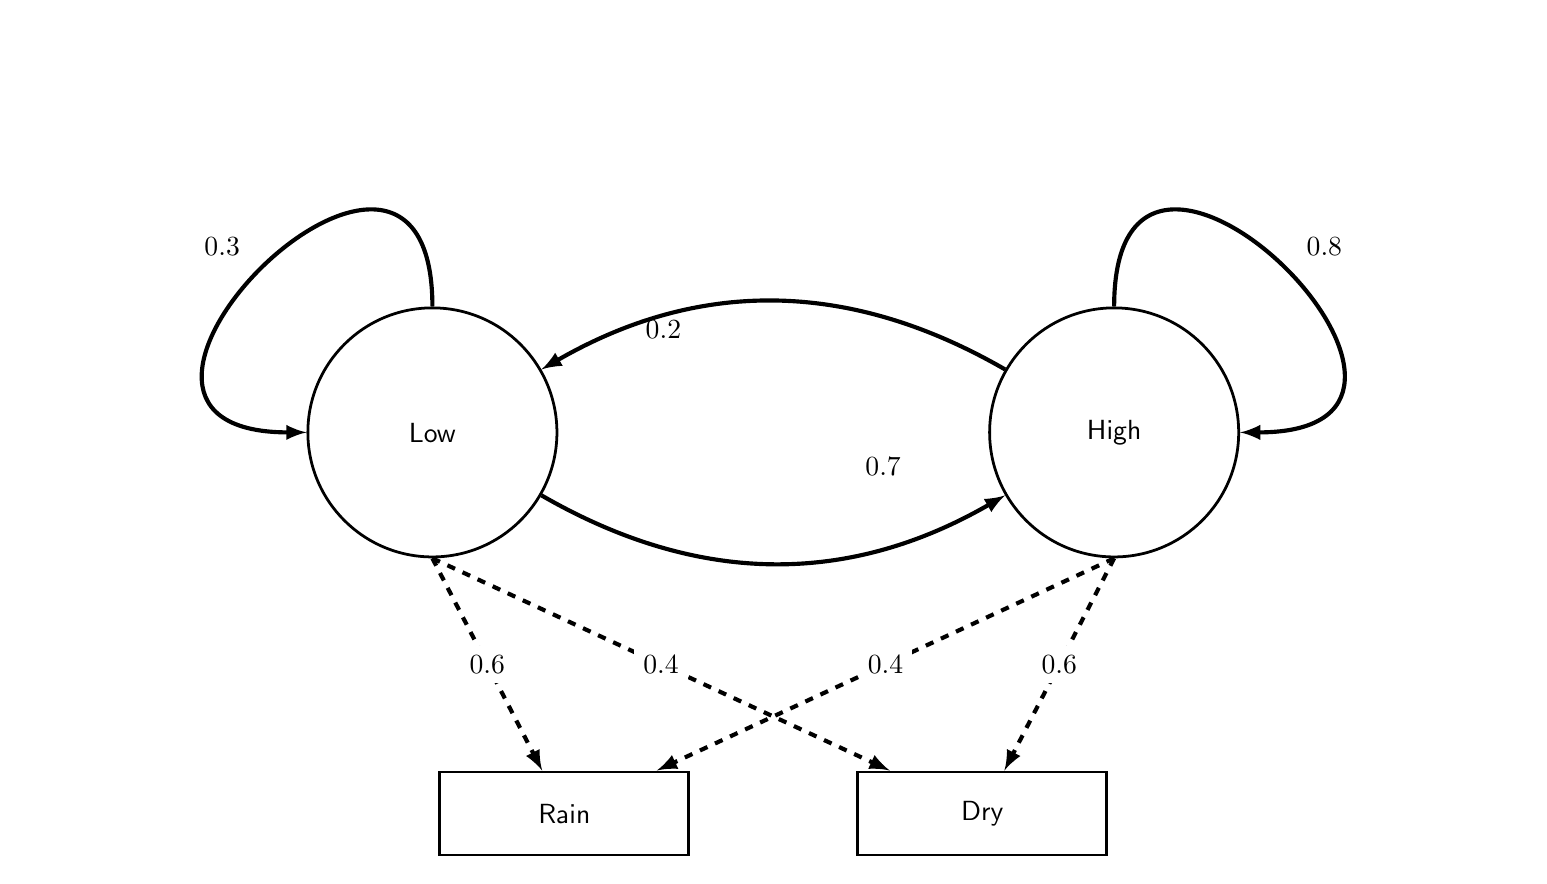
\begin{tikzpicture}
        \usetikzlibrary{shapes,arrows,positioning}
    % Define Styles
        \tikzstyle{block} = [rectangle, draw, fill=white, text centered, minimum height=3em, minimum width = 9em, line width = 0.1em]
        \tikzstyle{ellipse} = [circle, draw, fill=white, text centered, minimum height=3em, minimum width = 9em, line width = 0.1em]
        \tikzstyle{dashline} = [draw, -latex, line width=0.15em, dashed]
        \tikzstyle{curveline} = [draw, -latex, line width=0.15em]
    % Place nodes
        \node [block] (rain) {\sffamily{Rain}};
        \node [block, right = 6em of rain] (dry) {\sffamily{Dry}};
        \node [ellipse, above left = 9em and -3em of rain] (low) {\sffamily{Low}};
        \node [ellipse, above right = 9em and -3em of dry] (high) {\sffamily{High}};
    % Draw edges
        \path [dashline] (low.south) -- (rain) node [midway, fill=white] {0.6};
        \path [dashline] (low.south) -- (dry) node [midway, fill=white] {0.4};
        \path [dashline] (high.south) -- (rain) node [midway, fill=white] {0.4};
        \path [dashline] (high.south) -- (dry) node [midway, fill=white] {0.6};

        \path [curveline] (low) to[out=-30,in=-150] (high) node [below left = .5em and 7.3em] {0.7};
        \path [curveline] (high) to[out=150,in=30] (low) node [above right = 3em and 7.3em] {0.2};
        \path [curveline] (low.north) to[out=90,in=180, distance=10em] (low.west) node [above left = 6em and 2em, fill=white] {0.3};
        \path [curveline] (high.north) to[out=90,in=0, distance=10em] (high.east) node [above right = 6em and 2em] {0.8};
\end{tikzpicture}
}
%\includegraphics[width=3in]{figures/carl-schaefer/sketch-img002.jpg}
\end{center}

\caption{A hidden Markov Model}
\label{carl-schaeffer:fig:noisychmodel}
\end{figure}


The translation model suggested by TAP analysis can be formalized as a Hidden Markov Process in which a number of interconnected ``hidden'' states emit observations with a certain probability. \figref{carl-schaeffer:fig:noisychmodel} outlines the idea of a hidden Markov model, where the two hidden states (Low and High) emit possible observations (Rain or Dry) with a certain probability. A hidden Markov model can consist of a large number of hidden states and emit many different observations. The hidden states are organized in the form of (possibly completely connected) recursive networks and transition probabilities that indicate the likelihood with which one state follows another. A number of efficient algorithms exist to learn transition and emission probabilities from data and to compute most likely sequences of observations.

\subsection{Early and late stages of translation states}
\label{carl-schaeffer:sec:2.3}
\largerpage
 
\citet{DeGroot1992Determinants}, \citet{Hartsuiker2004}, \citet{Pavlenko2009} and \citet{Schaeffer2013Shared} assume that entries in the mental bilingual dictionary consist of nodes that link the lemmas, concepts, word forms and syntactical information between the two languages. The nodes are linked to all words that exhibit corresponding features in a language-independent fashion. They are, however, specific to particular language combinations as not all languages always realize the same morphosyntactic and semantic aspects in the same way. 

%Comment I am not sure I agree with this statement below (commented out). Shared representations are not a precondition for the possibility of translation: it is possible to establish links between items which are, in many ways, very different. I think our claim is that when shared representations exist, they facilitate the process which is what the second sentence says...

%The ability to translate texts between two different languages is based on the fact that these types of combinatorial nodes exist.
%I would also like to rephrase the sentence below thus (``some extent'' instead of ``large extent''):
%The models predict that the more nodes overlap between the source and \isi{target language} words and structures, the less time it takes to retrieve associations and to generate translations. This unchallenged \isi{translation process} is to some extent a subliminal process. 
The models predict that the more nodes overlap between the source and \isi{target language} words and structures, the less time it takes to retrieve associations and to generate translations. This unchallenged \isi{translation process} is to a large extent a subliminal process. 

The translation model by \citet{Schaeffer2013Shared} posits that the \isi{translation process} is \textit{recursive} given that translators often switch back and forth between source and target text in order to examine both texts for interpretive resemblance. In doing so, translators are primed by either the source or the target text, allowing them to register and analyze the resemblances in both texts. This view is in line with the \isi{monitor model} \citep{TirkkonenCondit2005} according to which an automatic default \isi{translation procedure} is interrupted when a problem occurs and triggers conscious translation processes.

%Comment
%maybe ``problem solving'' rather than ``conscious translation'' processes?
%In general, we need to be careful with the automatic/conscious distinction... Whether a process is truly automatic or whether it is conscious requires quite a bit of testing... Maybe it is better to talk about fast and slower processes, about early and late processes.






 
\figref{carl-schaeffer:fig:undist} visualizes an unchallenged \isi{translation process}. It shows a relatively undisturbed translation progression in which an English source sentence ``All of his victims were old weak woman'' is translated into \ili{Danish} ``Alle hans ofre var aeldre svagelige kvinder'' on the left and right axes respectively. Translation activities are depicted in the graph on a timescale, from ms 206.000 to 215.000. The overall translation of the eight words takes approximately 9 seconds. The figure shows keystrokes (insertions and deletions), gaze fixations on the source text (blue boxes with dots) and gaze fixations on the target text (green boxes with diamonds). 

\begin{figure}[h]
\includegraphics[width=\textwidth]{figures/carl-schaefer/sketch-img004.png}  
\caption{Example of an undisturbed translation progression}
\label{carl-schaeffer:fig:undist}
\end{figure}


  
Some of the measures for the translation segment in \figref{carl-schaeffer:fig:undist} are shown in \tabref{carl-schaeffer:tab:unchallenged} and explained as follows:

\begin{itemize}
\item \textit{FFDur}: \isi{first fixation} duration on the source word (blue rectangle)
\item \textit{FixS} and \textit{FixT}: number of fixations on the source text and target words respectively; there are only few fixations ($\le 10$) on each single word
\item \textit{TrtS} and \textit{TrtT}: \isi{total reading time} of source text word and its translation, respectively
\item \textit{Ins}, \textit{Del} and \textit{Dur}: number of counted insertions, number of counted deletions and total typing duration to produce the translation, respectively
\item \textit{Munit}: number of revisions (micro units) of a word (see page \pageref{carl-schaeffer:sec:4.4})
\item \textit{HTra}: \isi{word translation entropy} (cf. literality criteria 3, see page \pageref{carl-schaeffer:sec:4.1})
\end{itemize}

%comment: fpdurs is missing from this table...
\begin{table} 
\resizebox{\textwidth}{!}{\begin{tabular}{lrrrrrrrrrd{3}}
\lsptoprule
SToken	&	FFDur	&	FixS	&	TrtS	&	FixT	&	TrtT	&	Ins	&	Del	&	Dur	&	Munit	&	\multicolumn{1}{r}{HTra}	\\ \midrule
All	&	60	&	2	&	259	&	1	&	559	&	0	&	0	&	622	&	1	&	0.41	\\
of	&	0	&	0	&	0	&	1	&	559	&	5	&	0	&	622	&	1	&	0.74	\\
his	&	0	&	0	&	0	&	3	&	658	&	5	&	0	&	462	&	1	&	0.49	\\
victims	&	239	&	1	&	239	&	3	&	1177	&	5	&	0	&	634	&	1	&	0.49	\\
were	&	478	&	5	&	1116	&	1	&	80	&	4	&	0	&	445	&	1	&	0.00	\\
old	&	179	&	1	&	179	&	7	&	1136	&	6	&	0	&	1061	&	1	&	0.99	\\
weak	&	159	&	8	&	1796	&	5	&	1813	&	10	&	0	&	1177	&	1	&	1.36	\\
women	&	59	&	2	&	238	&	1	&	200	&	11	&	3	&	2234	&	1	&	0.24	
\\ \lspbottomrule
\end{tabular}}
\caption{Behavioural measures for smooth translation activities.}
\label{carl-schaeffer:tab:unchallenged}
\end{table} 



The segment in \figref{carl-schaeffer:fig:undist} is chararacterized by relatively few fixations on the source and target words and relatively short total reading times. There is a short delay between the reading of a source word and the production of the translation (i.e. the eye-key-span; see \citealt{Schaeffer2016Language}, \citealtv{SchaefferCarl}). Only the translation of ``weak'' and ``women'' required longer reading times, perhaps due to unusual character combinations in the \ili{Danish} translations.

\begin{figure}

\includegraphics[width=\textwidth]{figures/carl-schaefer/sketch-img005.png} 
\caption{Progression graph with complex patterns of monitoring behavior}
\label{carl-schaeffer:fig:challenged}
\end{figure}
 
 
\figref{carl-schaeffer:fig:challenged} shows an excerpt from an English $\rightarrow $ \ili{Chinese}  translation session, with much more complex patterns of ST and TT reading behavior, repeated regressions, re-reading, backtracking, deletions, revisions, etc. The production of this translation segment of 17 words took approximately 100 seconds, which is almost 5 times longer per word than the \ili{Danish} translation in \figref{carl-schaeffer:fig:undist}. The ST segment ``the extra green mile'' was read at least seven times, four times during an orientation phase between seconds 210 and 240 and then again three times during translation drafting. 

%comment: fpdurs is missing from this table...
\begin{table} 
\begin{tabular}{lrrrrrrrrd{3}}
\lsptoprule
SToken	&	FFDur	&	FixS	&	TrtS	&	FixT	&	TrtT	&	Ins	&	Del	&	Munit	&	\multicolumn{1}{r}{HTra}
\\ \midrule
the	&	183	&	2	&	316	&	0	&	0	&	0	&	0	&	0	&	1.35	\\
extra	&	234	&	20	&	5133	&	0	&	0	&	0	&	0	&	0	&	1.68	\\
green	&	267	&	24	&	8995	&	13	&	2683	&	2	&	0	&	1	&	0.46	\\
mile	&	250	&	6	&	2515	&	0	&	0	&	0	&	0	&	0	&	1.96	
\\
\lspbottomrule
\end{tabular}
\caption{Measures of challenged translation processes}
\label{carl-schaeffer:tab:challenged}
\end{table}

 
\newpage  
\tabref{carl-schaeffer:tab:challenged} lists the behavioural measures for the translation segment which was more challenging. In total, there were 20 and 24 fixations on the words ``extra'' and ``green'', respectively. The \isi{first fixation} durations \textit{FFDur} make up less than 5\% and 3\%, respectively, of the \isi{total reading time} for these words, indicating that most of the translation effort is related to later processes, such as source text integration or formulation of a translation hypothesis. In this example it seems that much effort was required to understand and/or formulate a first translation hypothesis for the phrase ``extra green mile'' since most of the reading occurred before the translation was typed.

\largerpage[-1] 
The words ``the'', ``extra'' and ``miles'' remain untranslated (\textit{Munit = 0}); only a \ili{Chinese} translation of ``green'' was produced and aligned.\footnote{Dashes `---' on the right Y-axes in the translation progression graphs indicate non-translated or non-aligned words for which there are no correspondances in the translation.} The relatively higher \textit{HTra} values indicate that translators have produced more different solutions for these words than for the translation of ``green''.

  
The available \isi{eye movement} measures seem to be well suited to capture unchallenged translation processes. However, existing measures are not well suited to describe the more complex reading patterns occurring during the later stages of challenged translation, because they either describe early processes (e.g. \isi{first fixation} duration or first pass \isi{reading time}) or they do not capture the time course of the late processes and very few measures describe the interrelationship between reading and writing activities (see also \citealt{SchaefferCarl}).
% While it is highly likely that a large amount of conscious processing has taken place during the translation production of this segment, the measures in the \tabref{carl-schaeffer:tab:challenged} are not sufficiently fine-grained to capture and describe the various hidden processes appropriately. 
%The available fixation measures seem to be well suited to capture processes of automated translation, they are rather undifferentiated with respect to more complex gazing patterns. While it is highly likely that a large amount of conscious processing has taken place during the translation production of this segment, the measures in the \tabref{carl-schaeffer:tab:challenged} are not sufficiently fine-grained to capture and describe the various hidden processes appropriately. 

%It is unclear how this observed behavior relates to translation strategies as isolated and described by TAP researchers. 




\tabref{carl-schaeffer:tab:earlylatemetrics} summarizes some of the existing measures. They will be explored in more detail in \sectref{carl-schaeffer:sec:4}. A distinction is made between reading measures which capture gaze activities, writing measures which describe typing processes and R\&W measures which describe how reading and writing are coordinated. These measures refer to sequences of the source and/or target texts, so-called Areas of Interest (AOI). AOIs are typically single words, phrases or sentences, and are characterized by the accumulated UAD as well as their linguistic and other annotations. The first pass \isi{reading time}, for instance, is the sum of fixation durations on a word (or another predefined text segment) from the \isi{first fixation} before the eyes leave the AOI again. The word \isi{production time} (\textit{Dur}, cf. page \pageref{carl-schaeffer:sec:4.1}) is the total time needed to type a word (i.e. a translation), including all its possible revisions. R\&W measures shown in \tabref{carl-schaeffer:tab:earlylatemetrics} can take values which may indicate early or late processes. 


\begin{table}
\begin{tabularx}{\textwidth}{p{1.5cm} X X p{1.5cm}}
\lsptoprule
					&	reading measures		&	writing measures					&	R\&W measures 	\\ \midrule
earlier processes	&	first-\isi{fixation duration}	&	keystrokes: insertions \& deletions	& \isi{eye-key span}		\\ 
~~~~~ $\vdots$		&	first pass \isi{reading time}	&	inter-key \isi{pauses}					&	~~~~~ $\vdots$ 	\\ 
~~~~~ $\vdots$		&	regression path duration&	micro units							&	parallel R\&W  	\\ 
later processes		&	\isi{total reading time}		&	revisions, word \isi{production time}		&	activities
\\\lspbottomrule
\end{tabularx}
\caption{Measures of the translation process}
\label{carl-schaeffer:tab:earlylatemetrics}
\end{table}

\subsection{A noisy translation processes model}
\label{carl-schaeffer:sec:2.4}

\begin{figure}[b]
\includegraphics[width=\textwidth]{figures/carl-schaefer/Noisy-TP-Model.png}
\caption{Observations, predictors and hidden variables in the noisy translation process model}
\label{carl-schaeffer:fig:noisytpmodel}
\end{figure}

A \isi{translation process model} taking into account hidden states of early and late processes is depicted in \figref{carl-schaeffer:fig:noisytpmodel}. The model resembles a Hidden Makov Model (HMM) in \figref{carl-schaeffer:fig:ncm} which consists of four levels of description. In the center is the \textit{Translator} who is constrained by a number of factors and who produces a sequence of behavioral patterns which lead to the final translation product. 

The \textit{Predictors} are a vast number of variables which are likely to play a role in the \isi{translation process} and which originate from an enormously heterogeneous field, including cognitive, linguistic, cross-linguistic, or textual, communicative and socio-cultural domains \citep{Toury2004}. Other researchers (e.g. \citealt{Risku2014}) also mention environmental conditions, including physical, geographic, economic, political and demographic aspects which might play a role in the \isi{translation process}. The \textit{Source Text} is another crucial predictor which will determine the characteristics of the target text.

The \textit{Translator} is modelled as a network of hidden states which implement the actual translation processes. In contrast to earlier hierarchical-stratificational models of translation \citep{Nida1964, Seleskovitch1975}, it is now generally accepted that there are states of early, automatic processes and states of more deliberate, strategic processing. \citet{Honig1991}, for instance, proposes a translation model which establishes a distinction between uncontrolled, associative \isi{translation competence} (i.e. unconscious early translation processes) and a controlled workspace in which micro and macro strategies are stored. The associative \isi{translation competence} corresponds to subliminal priming mechanisms, while the \isi{monitor} processes occur at a later stage as they require extensive conscious effort. 

 
The output of the model in \figref{carl-schaeffer:fig:noisytpmodel} has two levels of observations: \textit{product observations} capture the changes in the translation product, i.e. the sequence of intermediate texts that are produced during the \isi{translation process}. The final translation product is the final outcome in a series of successive intermediate text snapshots that emerge during the \isi{translation process} and the \isi{translation process} can be approximated by comparing the successive intermediate text snapshots. These observable textual changes are direct consequences of translators' activities which can be traced through logging technology.

Objective UAD such as keystrokes, mouse clicks, eye movements and other behavioral data can be recorded with keyloggers, eye-trackers and other tools, but  the collected UAD needs be segmented into meaningful \textit{behavioral patterns}. However, it is neither obvious how keystrokes and gaze data should be segmented, nor is it uncontroversial what the latent states are which emit those patterns.

The HMM in \figref{carl-schaeffer:fig:noisytpmodel} suggests that:
\begin{itemize}
\item the \textit{Translator} can be in only one state at any given time
\item translation processes are driven by a large number of \textit{Predictor} variables
\item there are probabilistic transitions between successive hidden states 
\item each state emits exactly one \textit{behavioral pattern} at each time
\item a \textit{behavioral pattern} produces a deterministic modification in the \textit{interim translation}
\end{itemize}

In \sectref{carl-schaeffer:sec:3} we will be concerned with the description and analysis of the behavioral patterns. The stream of UAD can be fragmented into segments of behavioral units which are suited to describe the \isi{translation process}. A Production Unit (PU), for example, is a coherent sequence of keystrokes where the lapse of time between successive keystrokes is below a given threshold, e.g., 1 sec. A PU can thus contain a single or a large number of keystrokes irrespectively how many words are produced. 

In \sectref{carl-schaeffer:sec:4} we argue that different hidden states can be related to different temporal aspects in which they are triggered. We discuss properties of earlier and later translation activities and hidden states in more detail.

\section{Patterns of translational behaviour}
\label{carl-schaeffer:sec:3}

This section discusses several approaches to fragment the UAD into sequences of behavioral patterns. Such patterns fragment the stream of translation activities on a temporal scale. We discuss units which capture gazing and typing data. In contrast to the behavioral data accumulated in textual AOIs, the UAD within the behavioral patterns may relate to several different textual items that may be at distant locations from each other. While there is a large repository of linguistic terminology to describe textual elements in AOIs --- such as PoS tags, linguistic functions etc. --- there are only very few approaches which fragment the \isi{translation process} data and little work has beed done to describe these units.


\subsection{Production units (PUs)}
\label{carl-schaeffer:sec:3.1}

\citet{Carl2016CRITT,Carl2011Gazing} define Production Units (PUs) as sequences of coherent keystrokes, where the pause between any two successive keystrokes is less than 1 second. A pause of more than 1000ms constitutes a PU boundary. PUs fragment the stream of translator activity data into sequences of coherent typing and \isi{pauses} that separate them. In contrast to a micro unit (see page \pageref{carl-schaeffer:sec:4.4}), a PU may stretch over several words, while a micro unit is defined as the flow of continuous typing that contributes to the production of one target word. A PU that stretches over $m$ words would thus be split into $m$ micro unit, where each produced word $1..._m$ is assigned its share of keystrokes. A word can be associated with several micro and production units, depending on how often it has been revised. A PU contains, among other things, the following information: 

\begin{itemize}
\item duration of the unit
\item duration of the preceding pause
\item number of insertions and deletions,
\item tokens involved in the source text and target text
\item average \textit{Cross} values
\item percentage of parallel source and target \isi{text reading} activity during unit production
\item degree of linear \isi{editing}
\end{itemize}

\citet{Singla2014} investigate to what extent post-editor profiles can be identified based on the information contained in PUs. They use data from five post-editors producing together 120 translations sessions which is contained in the LS14 study\footnote{ The data can be downloaded from \url{http://sourceforge.net/p/tprdb/svn/HEAD/tree/LS14/}}. They test several machine learning techniques but find that ``multilayer perceptron'' and ``classification via regression'' perform best for this task. Using 10-fold cross validation for classification, they achieve 46.48\% accuracy to identify post-editors which exceeds by far the baseline accuracy of 20\% which is based on guessing a post-editor by equal chance among the five participants.

\citet{Aziz2014} analyze PUs of post-edited texts, to investigate whether and how the properties of PUs are related to features of the sentences they appear in. Their investigation uses the CFT13 dataset\footnote{ The data can be downloaded from http://sourceforge.net/p/tprdb/svn/HEAD/tree/CFT13/} that was generated with the CASMACAT workbench \citep{Alabau2014}. PUs contain post-\isi{editing} information about number of insertions, deletions post-\isi{editing} time etc. \citet{Aziz2014} add further information to generate high dimensional feature spaces with nearly 100 features. The additional information included POS tags, named entities, chunk labels, and labels of semantic roles. The information was separated into PU level features and sentence level features ``such as the number of tokens in the sentence, the number of different phrases or the number of predicates and their arguments, which could indicate that the overall sentence is complex'' (179).

The authors use Principal Component Analysis (PCA) to visualize the high dimensional feature space and provide a detailed analysis of the data. \citet{Aziz2014} find that a correlation between sentence length and post-\isi{editing} time can be observed mainly in cases of low post-\isi{editing} activities. They find, for instance, that ``PUs involving verbs are slightly more time-consuming, while PUs related to nouns require slightly more typing'' \citep[189]{Aziz2014}. On the one hand, it is therefore ``possible to decouple sentence length from the difficulty of each PU in terms of how time-consuming and how many edits (character level insertions and deletions) it requires.'' \citep[189]{Aziz2014} On the other hand, a pause analysis becomes difficult, since ``the pause prior to \isi{editing} correlates very poorly to the character-level edits performed.'' \citep[187]{Aziz2014} It is unclear why a pause occurs and whether it is related to the successive typing events, as manifested in the PUs. This is supported by their finding that ``HTER correlates better with time and typing related to individual PUs than to cumulative sentence level indicators'' \citep[187]{Aziz2014}

With respect to \isi{editing} times, the authors find the following relations:
\begin{itemize}
\item there is a stronger correlation between insertions and duration than between deletions and duration
\item modal verbs, adverbs and coordinating conjunctions are more time consuming than gerunds and other non-finite verbs
\item pronouns take longer to post-edit than sequences of nouns and named-entities
\item consecutive NPs have a strong correlation with \isi{editing} duration and the preceding pause
\item the number of arguments in a sentence has an impact on its post-\isi{editing} duration
\end{itemize}

\citep[188]{Aziz2014} further find that ``there is very little correlation between the length of a sentence and how time-consuming individual PUs are''. In other words, post-editors process sentences in smaller units so that the post-\isi{editing} duration does not necessarily depend on properties of the whole sentence, and hence sub-sentence features may provide more informative cues about actual \isi{editing} effort than, for instance, sentence length. It is unclear whether and to what extent the findings for post-\isi{editing} carry over to from-scratch translation.

\citet[]{Schaeffer2016Language} attempt to predict concurrent ST reading and TT typing during from-scratch translation production. Their investigation is based on the assumption that ``instances of concurrent reading and writing during translation are indicative of automatic processes and shared representations''.They investigate concurrent activities in PUs using several possible predictor variables.They find that:

\begin{itemize}
\item the longer the PUs the more likely is concurrent reading activity
\item less concurrent reading is observed towards the end of the text
\item similarity of syntax in the ST and the TT facilitates concurrent activities
\item more experienced translators are more likely to show concurrent R\&W activities
\end{itemize}

The strong impact of the syntactic similarity on concurrent processing underpins their initial hypothesis that processes are likely to be more automatic when the ST and TT \isi{word order} is similar, as in this case primed, shared syntactic representations may more easily serve as the basis for TT production.

\subsection{Attention units (AUs)}
\label{carl-schaeffer:sec:3.2}

In order to compare the cognitive flexibility and processing automaticity of professional and student translators, \citet{Hvelplund2016} suggests to segment the translation activity data into attention units (AU).

Following \citet{Baddeley2007}, \citet{Hvelplund2016} argues that, on the one hand, cognitive flexibility is linked to planning, problem solving and decision making and involves the ability to focus and switch attention, or to divide attention simultaneously into several subtasks. Hvelplund further states that a translator with good cognitive flexibility will ``focus attention for precisely as long or short a period of time as is necessary only to those subtasks which are relevant to the successful execution of the translation task'' \citep[153]{Hvelplund2016}.


On the other hand, based on TAP studies \citep[e.g.][]{Jaaskelainen1991} it has been suggested that professional translators rely more on automatic processing than students. Translators' automaticity is, thus, closely related to experience.

In order to assess these hypotheses on the basis of translators' UAD, \citet[157]{Hvelplund2016} operationalizes the notion of \textit{attention unit} (AU) in the following way:

\begin{quote}
an AU is defined as uninterrupted processing activity allocated either to the ST (ST gaze activity), the TT (TT gaze activity and/or typing activity) or to the ST while typing (ST gaze activity and concurrent typing). Transitions to and from an AU indicate shifts in processing activity, and the point in time at which the transition occurs is used to identify the end of one AU and the beginning of the next AU. 
\end{quote}


He thus defines five AUs based on the following activities:

\newpage 
\begin{description}
\item[AU1:] ST reading
\item[AU2:] ST reading + typing
\item[AU3:] TT reading
\item[AU4:] TT reading + typing
\item[AU5:] Typing
\end{description}

While the cognitive flexibility is computed based on the durations of the AUs, the automaticity of the process is reflected in the pupil size where smaller pupil sizes indicate relatively less \isi{cognitive load} than larger ones. The pupil size for a AU was calculated as an average of all its gaze samples and a latency effect of 120 ms was factored into the calculation.

Based on an evaluation of the KTHJ08 data as shown in \tabref{carl-schaeffer:tab:tprmultilingdata} (see page \pageref{carl-schaeffer:tab:tprmultilingdata}), \citet{Hvelplund2016} finds that:

\begin{enumerate}
\item experienced translators spend more time on target text than less experienced translators.
\item a higher variability in AU duration by professional translators as compared to student translator indicating more flexibility and adaptability for the former group.
\item pupils are significantly larger for less experienced translators than for experienced translators.
\end{enumerate}

Further, in order to assess the \isi{translation process} flow, Hvelplund counts all the transitions between any two successive AU labels, separately for professional and student translators, and stores them in a  $5 \times 5$ transition matrix. He compares the two matrixes and observes that experienced translators shift from AU1 (ST reading) in 65.5\% of the cases to typing activity (either of AU2, AU4 or AU5) while student translators do this only in 52.2\% of the cases. Student translators switch to AU3 more often than professionals, which suggests that students aim more often at confirming meaning hypotheses (reflecting some kind of uncertainty), rather than allocating the cognitive resources directly to TT typing once a meaning hypothesis has been established.

\subsection{Actvity units}
\label{carl-schaeffer:sec:3.3}

Not unlike \citet{Hvelplund2016} AUs, \citet{Carl2016CRITT} suggest to fragment the activity data into seven different types of segments with the following labels:

\begin{description}
\item[Type1:] Reading the source text (ST)
\item[Type2:] Reading the target text (TT)
\item[Type4:] Typing activity
\item[Type5:] Typing while reading ST
\item[Type6:] Typing while reading TT
\item[Type7:] Typing while reading ST and TT\footnote{In more recent work, this type of unit is decomposed into units of type 1,2,4,5,6 or 8}
\item[Type8:] No activity recorded
\end{description}

Type1, Type2 and Type4 are basic translation activities. Type5 to Type7 take into account that source and target \isi{text reading} can occur concurrently with typing, and a Type 8 is assigned to segments if no activity is logged for longer than a given threshold. \figref{carl-schaeffer:fig:cuunit} shows the segmentation of a translation segment into AU units. The data is identical to that in \figref{carl-schaeffer:fig:undist} 5 but AU boundaries are marked. 

\begin{figure}

\includegraphics[width=\textwidth]{figures/carl-schaefer/sketch-img011.png} 

\caption{Translation session fragmented into CU units}
\label{carl-schaeffer:fig:cuunit}
\end{figure}

\figref{carl-schaeffer:fig:cuunit} shows a long ST reading activity (Type1, in blue) of approximately 30 seconds, between seconds 208 and 238, followed by a number of shorter \isi{pauses} (Type8, in black), TT reading (Type2, in green) and typing activities (Type4, in pink) etc. These segments describe exhaustively the \isi{translation process} and the properties of the sequence might be significant for certain types of translators and/or translation strategies.

In order to assess to what extent the profiles of machine-translation post-editors can be detected from the labels of the AU, \citet{Singla2014} investigate units of Type4 and Type8 (i.e. typing and \isi{pauses}) of five post-editors with different amounts of experience. They use data from 120 translations sessions which are extracted from the LS14 study\footnote{The data can be downloaded from \url{http://sourceforge.net/p/tprdb/svn/HEAD/tree/LS14/}} and subdivide Type 4 and Type 8 units into five categories based on their durations. They compute a trigram language model of activity sequences for each post-editor and compute a transition matrix which is filled with the perplexity scores of each post-editor's language model on the other post-editor's activity sequences. A discriminative classifier is then used to cluster post-editors into two classes on the assumption that the events that make up the \isi{translation process} provide enough information for the individualization of post-editor profiles.

\citet[56]{Singla2014} find that ``experienced post-editors produce similar kinds of activity sequences in contrast with the activity sequences of inexperienced post-editors''. They also notice that post-editors with a similarly negative attitude towards post-\isi{editing} tend to have similar activity patterns.

\citet{MartinezGomez2014Characterization} use a subset of 204 sessions from the data shown in \tabref{carl-schaeffer:tab:tprmultilingdata} that is annotated with information about translator experience and certification: 99 of the 204 sessions were produced by 47 non-certified translators, and 105 sessions were produced by 47 certified translators. They report that:

\begin{quote}
translators engage 14\% of their time in source \isi{text reading}, between 17\% to 37\% in target \isi{text reading}, between 35\% to 42\% inserting characters and 4\% deleting characters. Certified translators spent significantly larger proportions of time in target \isi{text reading} and target text typing than non-certified translators. The most common translation activity was the concurrent combination of ``source \isi{text reading}'', ``target \isi{text reading}'' and ``target text typing'', which occurred around 45\% of the time for non-certified translators and 65\% of the time for certified translators. \citep[n.p.]{MartinezGomez2014Characterization}
\end{quote}

In an extension of this experiment, \citet{MartinezGomez2014Recognition} use the same data to recognize translator expertise, based on the assumption that ``Translators have different perceptual and motor activities, depending on their level of expertise.'' They compare two methods to assess this hypothesis, one based on the AUs, and another one using unsupervised machine learning techniques with a view to discover regularities in the logging events and to reveal latent activities, that would otherwise not be detected.

For the unsupervised learning method, each log event (fixation and keystroke) was enriched with 31 additional features that were extracted from the  immediate context, such as the number of insertions, deletion and fixations within the past and the next 10 events, together with the time offsets from the current event. The information was stored in the form of vectors which were then classified using a k-means clustering method (3 to 8 classes). Tri-gram language models were built from the sequences of cluster labels, and random forests used to predict translator expertise, such as whether the user is a certified translator or not (binary classification), his/her years of training (regression) and years of experience (regression).

\citet{MartinezGomez2014Recognition} report an error reduction in the recognition of certified translators, and moderate but significant error reductions in the recognition of years of experience, as compared to a baseline. Best results were obtained with the unsupervised technique. They also report that CU unit of type 5 (i.e concurrent ST reading and typing) is more likely for certified translators than for non-certified translators.

\subsection{OST units}
\label{carl-schaeffer:sec:3.4}

\begin{figure}
 \includegraphics[width=\textwidth]{figures/carl-schaefer/sketch-img012.png} 
\caption{Annotation of OST units}
\label{carl-schaeffer:fig:ost}
\end{figure}

Another approach to fragmenting the process data was suggested by \citet{Nitzke2016}. They manually annotate the activity data into two main categories, orientation (O) and \isi{revision} (R) with five sub-categories:

\begin{itemize}
\item \textit{Ost}: The participant spends time reading both source and target text
\item \textit{Os}: More than 80 \% of the fixations were on the source text
\item \textit{Ot}: More than 80 \% of the fixations were on the target text
\item \textit{Rl}: Every word or phrase is processed only once.
\item \textit{Rs}: The participant works on a part of the text, moves on but jumps back later to readjust the parts she already worked on.
\end{itemize}

With five sub-classes the annotation schema is less complex than the CU activity units - and much coarser grained. The translator activity data of 406 segments has been manually annotated into 985 segments, which is on average slightly more than two OST units per segment. 


In an attempt to automatically detect OST units, \citet{Laubli2016} segment the process data into fragments of 3 seconds, and assemble all process events (keystrokes, mouse clicks, ST fixations and TT fixations) for each segment in a vector of observations. Similar to the method used by \citet{MartinezGomez2014Characterization}, the observation vectors are then classified with a k-means clustering method and a \isi{Hidden Markov model} (HMM) is trained on the sequences of cluster labels and observation vectors. The assumption is that the cluster labels represent the underlying states of the OST annotation (orientation, \isi{revision}, and, as an additional state, also pausing) where each state produces randomly an observation. The transition probabilities in the HMM and observation probability densities are then trained based on the available data. The aim of the model is to yield the most probable label for each observation, taking into account (i) the feature values (dimensions) of the current observation and (ii) the label assigned to the preceding observations. In a final step the cluster labels are mapped on the three OST labels: orientation, \isi{revision} and pause. The authors show that the system reaches as high an accuracy to predict the times spent on orientation, \isi{revision} and pause as some of the human annotators.

\subsection{Conclusion}
\label{carl-schaeffer:sec:3.5}

This section summarizes different methods of segmenting the UAD into successive chunks. Depending on the available logging data, most of the segmentation methods make use of cues in the data, such as \isi{text production} \isi{pauses} and/or the location of the gaze data on the source or target text to define segment boundaries. An exception is the segmentation method by \citet{Laubli2016} who segment the UAD into chunks of 3 seconds duration. With the exception of OST units described in \sectref{carl-schaeffer:sec:3.4}, all segmentation methods work fully automatically.

The reported investigations show that some segment properties are typical for different translator profiles and degrees of translator expertise. They are are also indicative of various translation problems.

The research discussed in this section can be characterized as instances of probabilistic translation modelling as discussed in \sectref{carl-schaeffer:sec:2.1} and equation \ref{carl-schaeffer:eqn:tp} on page \pageref{carl-schaeffer:eqn:tp}. Models are sought which predict behavioral patterns based of a number of different predictor variables. Linguistic features of the source text are investigated with respect to their effect on production times and \isi{revision} behavior, patterns of reading and writing are related to cognitive models of the translator, such as translation expertise, and different translation techniques, \isi{machine translation} and from-scratch translation are assessed in relation to translation effort.

Pause analysis is perhaps the most common approach for the analysis of behavioral patterns. In pause analysis it is assumed that longer \isi{pauses} between successive keystrokes signal higher \isi{cognitive effort}. \citet{Obrien2006} analyses keystroke \isi{pauses} in post-\isi{editing} and suggests that analyzing \isi{pauses} is a useful indicator of \isi{cognitive effort} in post-\isi{editing}. \citet{Immonen2006} finds that in translation, pause length is higher at word and clause boundaries. \citet{Lacruz2012} introduce average pause ratio as a metric to establish a relationship between \isi{pauses} and \isi{cognitive effort} in post-\isi{editing}. 

However, to obtain a more complete picture of the \isi{translation process}, we ought to investigate the translators' ``black box'' in more detail. In the next section we will therefore investigate properties of the translators' hidden states, which, according to the Noisy Channel Model in \sectref{carl-schaeffer:sec:2.4} emit behavioral patterns.




\section{Hidden translation states}
\label{carl-schaeffer:sec:4}

It is unclear how many hidden translation states can or should be distinguished that participate in the \isi{translation process}. However, a distinction can be made between states which are triggered through early priming mechanisms and other more time-consuming and late(r) states which involve more cognitively demanding problem solving strategies. The TP model suggested in \figref{carl-schaeffer:fig:noisytpmodel} distinguishes these states into ``early'' and ``late'' states. 

Priming is an unconscious mechanism that is based on the implicit memory of a first (source) stimulus which carries over to a subsequent, target stimulus and which has an impact of the execution of a following task. It has been shown that \isi{bilinguals}, and therefore also human translators, use implicit memories during language production. Priming effects exist between stimuli in different modalities, such as visual and verbal. They are, however, stronger if source and target stimuli are in the same modality, e.g. within written language. Priming effects can be observed in translation and in post-\isi{editing} of \isi{machine translation} output (PEMT), but --- as we will show --- the effects are more noticeable in PEMT, presumably due to the fact that priming effects are generally stronger within one language (i.e. the MT output and final translation) than between two languages \citep{Pickering2008}. 


%Comment: neither Jensen et al (2009), nor Ruiz et al manipulate choice... Why don't we cite our entropy study here?
The degree of similarity between source and target items has an effect on the strength of the priming effect -- the greater the similarity, the stronger the priming effect. Priming facilitates and simplifies translation. Priming effects exist for the choice of words as well as for word
order. \citet{Jensen2009Distribution} and \citet{Ruiz2008Activation} report shorter ST reading times in translation if the \isi{word order} in the ST is identical with the \isi{word order} in the TT. \citet{Schaeffer2016Word} report longer reading times for words with more possible choices than for words with fewer choices. This result is in accordance with Campbell's Choice Network Analysis \citep{Campbell2000}: The more choices translators have in the selection of a translation, and the more complex the decisions are that they have to make, the more difficult the translation will be. Simpler translational decisions often lead to identical results while more variation in the traslation often implies difficult more difficult decisions.

%Comment: I find this problematic - the process data does not encode, it records. and what it records is behaviour. We hypothesise that this behaviour is the result of automatic and conscious process.
%As shown in Figures \ref{carl-schaeffer:fig:undist} and \ref{carl-schaeffer:fig:challenged}, \isi{translation process} records traces of early, fast and later, slower translation behavior. Early behavioural measures are likely be evidence of automatised processes, while later, more time-consuming processes are likely to involve more conscious problem solving activities. 
As shown in Figures \ref{carl-schaeffer:fig:undist} and \ref{carl-schaeffer:fig:challenged}, \isi{translation process} data encodes traces of early, automatized and later translation behavior. Automatised processes occur quickly and leave their traces early on, while later, more time-consuming processes are likely to involve more conscious problem solving activities. 

A \isi{noisy channel model} of translation as depicted in \figref{carl-schaeffer:fig:noisytpmodel} takes into account various kinds of hidden processes which ought to explain and generate the traces in the observed UAD. This section summarizes a few constraints of the hidden states, related to the observable output of early and later processes. 

A large amount of research exists that investigates conscious processes in translation \citep[e.g.][]{Jaaskelainen1991,Loerscher2005}.  According to \citet{Gutt1989}, the translator's task is to recode the source text into a \isi{target language} text in such a way that interpretive resemblance in regard to explicatures and implicatures of both texts is achieved. In order to examine interpretive resemblance, translators consciously apply meta-cognitive monitoring processes. 
Gutt's theory builds on relevance theory \citep[RT,][]{Sperber1995}, which posits that linguistic forms encode semantic representations that are recovered using unconscious, automatic decoding processes. As a pragmatic theory of communication, RT seeks to explain the inference procedures that build on the automatic encode-decode mechanism and on which successful communication relies. The  distinction between the process of encoding-decoding messages and the process of making inferences from evidence coincides for  \citet{Blakemore2002} with  the distinction between semantics and pragmatics: linguistic semantics provides logical forms which are taken as input by pragmatic inferences constrained by the principle of relevance. 

This section aims at giving empirical evidence for the existence of early and late translation processes. In \sectref{carl-schaeffer:sec:4.1} we describe the experimental material that much of the successive sections rely on.  
%In \sectref{carl-schaeffer:sec:4.3}, we report evidence for the existence and importance of early processes in the \isi{translation process}. Traces of these processes are captured by \isi{first fixation} duration.
In \sectref{carl-schaeffer:sec:4.2}, we investigate linguistic parameters that have an effect on the word production duration. Production duration is a possible indicator of translation difficulty and the amount of priming and more time-consuming translation strategies that went into the production of a translation. We show that, among other parameters, the number of possible translations for a word is a strong indicator of translation difficulty, which has an impact on early as well as late translation processes. In \sectref{carl-schaeffer:sec:4.3} we have a closer look at syntactic properties of lexical variation in the translation product in from-scratch translation and in post-\isi{editing}. Finally in \sectref{carl-schaeffer:sec:4.4} we discuss \isi{revision} behavior, which accounts probably for the latest of the translation processes.


\subsection{Experimental Material, Measures and Metrics}
\label{carl-schaeffer:sec:4.1}

\begin{table}
\begin{center}
\begin{tabular}{lrllrrrrr}
\lsptoprule
Study	&	Sessions&TL&\textit{Task}&\textit{Texts}&\textit{Part}&\textit{FDur}	&\textit{KDur}&\textit{TT Tok}	\\ \midrule
TDA		&	48	&	en	&	C	&	1-6	&	15	&	6.1	&	5.8	&	6792	\\
\tablevspace
KTHJ08	&	69	&	da	&	T	&	1--3	&	24	&	6.4	&	5.5	&	10571	\\
\tablevspace
SG12	&	45	&	de	&	P	&	1--6	&	23	&	5.6	&	1.9	&	6352	\\
\tablevspace
SG12	&	47	&	de	&	T	&	1--6	&	24	&	9.4	&	4.6	&	6632	\\
\tablevspace
BML12	&	64	&	es	&	P	&	1--6	&	32	&	2.3	&	0.9	&	9012	\\
\tablevspace
BML12	&	63	&	es	&	T	&	1--6	&	32	&	8.2	&	5.8	&	8936	\\ 
\midrule
total	&	336	&	4	&	3	&	6	&	150	&	38	&	24.5&	48295	\\
\lspbottomrule
\end{tabular}
\end{center}
\caption{Annotated data for the syntactical entropy study}
\label{carl-schaeffer:tab:tprmultilingdata}
\end{table}

\largerpage[-1]
\tabref{carl-schaeffer:tab:tprmultilingdata} gives an overview of the size and number of texts. A total of 336 target texts (TTs) with a total of 48.295 \isi{target language} tokens (TT Tok) were produced from six different English source texts (ST) into four target languages, \ili{Danish} (da), \ili{German} (de), \ili{Spanish} (es) and English (en). The English TTs resulted from a copying task (C), English to English, whereas the other texts were either post-edited (P) or translated (T). The translations were produced by 95 translators over a period of 38 hours (\textit{FDur}). The column \textit{KDur} shows the accumulated keying time, excluding production \isi{pauses} of more than one second. Note that the ratio of keying time (\textit{KDur}) vs. total \isi{production time} (\textit{FDur}) is much smaller for post-\isi{editing} than for from-scratch translation, and even less in the copying task. \ili{Danish} translations were only produced for three texts (1-3). The column \textit{Part} indicates the number of different participants involved in each translation study. 

 
\largerpage[-1]
From the logs of these sessions, a number of features were extracted, (cf. \citealt{Carl2016CRITT}), among others:
\begin{itemize}
\item \textit{LenS}: length of the English source text word in characters
\item \textit{LenT}: length of the translation in characters
\item \textit{STseg}: (sequential) number of the source text segment
\item \textit{Prob1}: frequency of the English source text word (according to BNC) 
\item \textit{PoS}: English source texts were part of speech (PoS) tagged. \tabref{carl-schaeffer:tab:postags} gives an overview of the used tagset.
\item \textit{Dur}: translation duration is the amount of time needed to produce the translation of a word. 
\item \textit{HTra}: \isi{word translation entropy} 
\item \textit{Cross}: distance between the English source text word and its translation 
\end{itemize}

In order to assess the literality of a translation, \citet{Carl2016CRITT,Carl2016Literality} introduce a literality metric which measures the similarity of a source text (ST) and its translation, the target text (TT), along the following three criteria:

\begin{itemize}
\item ST and TT segments have the identical \isi{word order}
\item ST and TT words are one-to-one translation equivalences
\item ST words have one (preferred) translation in the context
\end{itemize}

Literality criterion (2) is met if each word in the ST corresponds to exactly one TT word and vice versa, while criterion (1) is realized if the translation equivalents occur in the same order in the ST and in the TT. These two criteria are represented by an integer value, referred to as \textit{Cross} and relate to the amount of crossing word alignments (inter-lingual alignment distortion). A one-to-one correspondences results in a \textit{Cross} value of 1, and this value grows (negatively or positively) with the distance between the aligned words.  Approximately 40\% of all words in the TPR-DB (English STs) have a \textit{Cross} value greater or smaller than~1 \citep[190]{Schaeffer2016Word}. 

In order to assess literality criterion (3) we use a corpus of word-aligned, alternative translations and measure the entropy of the translation realizations. This measure is referred to as \isi{word translation entropy} \textit{HTra}. Approximately 90\% of all words in the TPR-DB (English STs) have more than one translation alternative, and thus a value   $\textit{HTra} > 0$ \citep[190]{Schaeffer2016Word}.

\subsection{Production duration in translation and post-editing}
\label{carl-schaeffer:sec:4.2}

The reduction of translation duration (the increase of productivity) is a driving force for much of the technological development of \isi{machine translation} (MT) and for post-\isi{editing} of \isi{machine translation} (PEMT). While it has been shown in several places that PEMT is often quicker than from-scratch translation \citep{Plitt2010,Obrien2014PostEditing}, it has not often been investigated what the possible determining factors, and what the impact for on the translation product are. 

To test which properties of the text might have an impact on the translation duration, we analysed six English texts from studies BML12 and SG12, (see \tabref{carl-schaeffer:tab:tprmultilingdata}). We extracted 15,313 ST and 15,568 TT words that were translated into \ili{Spanish} and \ili{German} by 32 and 24 translators respectively and they were also post-edited into \ili{Spanish} and \ili{German} by 32 and 23 translators, respectively. The data was analyzed using R (R Development Core Team, 2014) and the lme4 \citep{Bates2014} and languageR \citep{Baayen2013} packages to perform linear mixed-effects models (LMEMs). To test for significance, the R package lmerTest (Kuznetsova, Christensen, \& Brockhoff, 2014) was used, which implements ANOVA for mixed-effects models using the Satterthwaite approximation to estimate degrees of freedom. The final model included participant, ST token, text and \isi{target language} as random variables. The predictor variables were ST token frequency (\textit{Prob1}), word length of the ST token in characters (\textit{LenS}), \textit{Cross} and \textit{HTra}, in addition to task, i.e. post-\isi{editing} and translation, as an interaction with both \textit{Cross} and \textit{HTra}. The dependent variable, \isi{production time} per word (\textit{Dur}) was log transformed, because it was not normally distributed. Data points which were more than 2.5 standard deviations below or above a participant's mean were excluded (3\%). All effects were highly significant (all \textit{t} {\textgreater} 3 and all \textit{p} {\textless} .001).

 
The translation duration \textit{Dur} indicates the \isi{production time} for a translation. It is also an indicator of earlier and later processes: the more time is needed to produce a translation, the more likely will the translator be involved meta-cognitive reasoning. As shown in \figref{carl-schaeffer:fig:stfreq} the production duration dependes on a number of additional factors.

\begin{figure}[p] 
\includegraphics[width=\textwidth]{figures/carl-schaefer/HTRA_Cross_TRA_PE_DUR2.pdf} 
\caption{The effect of source text frequency (\textit{Prob1}), ST word length in characters (\textit{LenS}), word
translation entropy (\textit{HTra}) and word order differences (\textit{Cross}) on gg{production time} (\textit{Dur}) and
observed translation variants for post-editing (P) and translation (T).}
\label{carl-schaeffer:fig:stfreq}
\end{figure}

\figref{carl-schaeffer:fig:stfreq} shows the effect of \textit{Cross} and \isi{word translation entropy} (\textit{HTra}) on word \isi{production time} \textit{Dur}. The Figure shows that post-\isi{editing} is much quicker for words which have small \textit{Cross} and \textit{HTra} values. Post-\isi{editing} may take as long as from-scratch translation if the MT output is modified (i.e. many different variants are produced) and/or for large \textit{Cross} values.

It is possible that MT systems produde more acceptable translations for segments in which the \isi{word order} is similar (i.e. \textit{Cross} values are low) than for segments in which a large amount of syntactic reordering is required. In turn post-editors would need to produce less modifications for translations with low \textit{Cross} values which would explain why post-editors take less time to produce these words as compared with words which have a very different position in the TT, in relation to the ST. 


\subsection{Variation in translation and post-editing}
\label{carl-schaeffer:sec:4.3}

The amount of different translations that are possible for a word (\textit{HTra}) has a strong effect on \isi{production time}. In this section we investigate this phenomenon in more detail. 
%Interferences of grammatical and/or lexical structures from the \isi{source language} to the \isi{target language} exist in
%translation (e.g. \citet{toury1979,eskola2004,Baumgarten2008,Becher2009The}) as well as in PEMT.
Post-editors seem to be less creative than translators; often, they do not modify the MT output which leads to fewer variants in the translation product than during from-scratch translation. 

\citet{Culo2014}, for instance, describe a study in which 12 professional translators and 12 translation students translate or post-edit six texts from English (L2) to \ili{German} (L1). \citet{Culo2014} discuss the following MT output in detail:

\begin{itemize}
\item[EN]: \textit{In a gesture} sure to rattle the \ili{Chinese} Government
\item[DE]: \textit{In einer Geste}, die die chinesische Regierung wachrüttelt 
\end{itemize}


The \ili{German} translation ``\textit{In einer Geste}'' is understandable but not idiomatic. It is a literal one-to-one translation -- according to criteria 1 and 2 above -- which was generated by an MT system but which was rarely changed by the post-editors. However, a great variation of different idiomatic versions was found in human translations of the same text segment. Human from-scratch translations for the above example include: ``Als Geste'', ``Es ist eine Geste'', ``Mit der Absicht'', ``Als Zeichen des Widerstandes'' and ``Mit einer Aktion''. The eight translators who translated this text produced seven different versions, while seven post-editors only came up with three different versions. The example clearly shows that translators are more creative, resulting in more diverse translation solutions and thus high \textit{HTra} values, while post-editors are more heavily primed by and biased towards the solutions generated by the MT system which results in low \textit{HTra} values but also faster production times. Note also that the translation \textit{In a gesture} $\leftrightarrow$ \textit{In einer Geste} can be aligned word-by-word, which is not the case for most of the from-scratch translations.

\begin{figure}
\begin{center}
\includegraphics[width=4in]{figures/carl-schaefer/PerplexityPoS-DE.png} 
\includegraphics[width=4in]{figures/carl-schaefer/PerplexityPoS-ES.png} 
\end{center}

\caption{Priming in translation (TRA) and post-editing (PE). Perplexity in word translations exhibits the variation of generated target texts, which is always higher in translation from scratch than in post-editing.x}
\label{carl-schaeffer:fig:primtra2}
\end{figure}


Tightly connected to the phenomenon of interference is the amount of variation in translation solutions. \figref{carl-schaeffer:fig:primtra2} shows \isi{word translation} perplexity from English to \ili{German} and English to \ili{Spanish} for different word classes (PoS tags, see \tabref{carl-schaeffer:tab:postags}, below). The texts were extracted from the SG12 and BML12 studies (see \tabref{carl-schaeffer:tab:tprmultilingdata}) and contain approximately 800 source text words. The degree of translation variance can be measured as perplexity: an even distribution of several realised translations (e.g. all translators generate a different translation) leads to high perplexity values, while an uneven distribution (i.e. many translators generate the same translation) does not. 

The values for post-\isi{editing} and original translation are indicated. Some PoS tags, such as e.g. JJS (superlative e.g. ``largest'', ``least''), NNP (proper names), CC (conjunctions) only produce a very small number of translation alternatives (low degree of perplexity). Other PoS tags, such as e.g. RP (particles), VBN (participles) exhibit more variation in the target text. In any case, the degree of \isi{word translation} perplexity in post-\isi{editing} is always lower than in translation from scratch. As pointed out in \sectref{carl-schaeffer:sec:4.3}, this is presumably due to the fact that MT output is often accepted without changes and all post-editors therefore often accept the same word translations.

Some PoS tags in the \ili{Spanish} translation exhibit more variation than the \ili{German} translation. For example, there is less variation in the translation of superlatives (JJS) in \ili{German} while there is a relatively large amount of variation in the \ili{Spanish} translation. Other word classes (e.g. conjunctions) seem to be translated in the same way by most translators and post-editors. The difference between post-edited texts and translations from scratch, however, are more pronounced for \ili{Spanish} than for \ili{German}. This suggests that \ili{Spanish} post-editors accept MT output more frequently than \ili{German} post-editors. 


\subsection{Translation revision}
\label{carl-schaeffer:sec:4.4}

According to \citet{Gutt1991} the aim of a translation is to achieve appropriate contextual effects in the \isi{target language} without unnecessary effort for the reader of the target text, so that the translation corresponds to the original source text in terms of relevant aspects. In order to achieve this goal, translators consciously keep track of the possible associations between stimulus, context and interpretation, so that the resulting translations obey to the principle of cognitive and communicative relevance \citep[260]{Sperber1995}.

Translation \isi{revision} is in many cases a compulsory activity to generate intelligible and optimal relevant translations. A distinction is made between other-\isi{revision} and self-\isi{revision}. Other \isi{revision} is carried out by someone other than the translator, while self-\isi{revision} (or checking) is done by the translator him- or herself. Self-\isi{revision} of a translation is an integral part in the translators' \isi{translation process}. \citet{Jakobsen2003} distinguishes between online \isi{revision}, i.e. \isi{revision} during the translation drafting process, and 'end \isi{revision}', which occurs after the completion of the first draft without delay. According to \citet[109]{Mossop2007Revising}, \isi{revision} may be defined as ``that function of professional translators in which they identify features of the draft translation that fall short of what is acceptable and make appropriate corrections and improvements''. Revisions may be due to problems in transfer, content, language and presentation \citep{Mossop2007Revising} and may take place in translators' minds during the decision-making process (`internal \isi{revision}') or appear on paper or the computer screen when actual changes are being made (`external \isi{revision}', \citealt{Kunzli2007}). 

Relevance Theory considers words and phrases to encode procedural components that contain instructions which control procedures that limit calculations of conceptual representations. This distinction is known as conceptual and procedural encoding. Procedural encoding thus guides the conceptual computations and leads to processes of comprehension so that the reader may work with a conceptual representation \citep{Blakemore2002}. In accordance with these observations, \citet[16]{Sperber1993} note that ``conceptual representations can be brought to consciousness; procedures cannot. We have direct access neither to grammatical computations nor to the inferential computations used in comprehension.'' 

However, according to \citet{Alves2003Triangulating}, translators consciously learn how to manipulate conceptually and procedurally encoded information. They suspect that conceptually encoded information is easier to translate than procedurally encoded information as conceptual encoding exhibits a ``relatively stronger interpretive resemblance between source and target texts'' (p 20). \citet{Sekino2012} reports findings based on translation data for \ili{Japanese} into \ili{Portuguese}. Their results corroborate \citet{Alves2003Triangulating}, showing that processing effort is greater when dealing with procedural encodings in both from-scratch translations and in post-\isi{editing} tasks in terms of keystrokes, fixation counts and \isi{fixation duration}.

In order to assess these findings with our data, we investigate ST reading patterns and TT \isi{revision} patterns on a set of UAD which included that shown in \tabref{carl-schaeffer:tab:tprmultilingdata}. The duration of the fixations -- and also of the \isi{first fixation} -- signals the \isi{cognitive effort} for processing a word. Fixations tend to be longer on words that require effortful processing as, for instance less frequent words, words containing spelling errors, ambiguous words, words which are inappropriate in a given context, etc. \citet[e.g.][413]{McConkie2003}.

We adopt \citet{Alves2011On} notion of micro units to quantify the amount of self-\isi{revision}. A micro unit (\textit{Munit}) is a typing burst which contributes to the translation of an ST token and which does not contain inter-keystroke \isi{pauses} of more than 1 second. An \textit{Munit} --- in the way we use it here --- indicates how the translation of a source word was modified. The number of \textit{Munits}  that the translation of a word is involved in is thus an indicator for its translation effort, since each revolving modification is an indicator for restructuring or reconsidering the translation a larger context.

We PoS-tagged the English source texts\footnote{we used the Penn treebank PoS tagset \url{https://www.ling.upenn.edu/courses/Fall\_2003/ling001/penn\_treebank\_pos.html}} and investigated their translations into \ili{Danish}, \ili{German}, \ili{Spanish}, Estonian, \ili{Chinese}, and Hindi (i.e. the studies ACS08, BD08, BD13, BML12, HLR13, KTHJ08,MS12, NJ12 and SG12 (cf. \citealt{Carl2016CRITT})) with the hypothesis that:

\begin{enumerate}
\item procedurally encoded words in the English source texts would require relatively more \isi{reading time}
\item their translations into the target languages would require more \isi{revision} time than conceptually encoded words
\end{enumerate}



To this end, we classified the English PoS tags into 2 bins, labeled \textit{conceptually encoding} and \textit{procedural encodings}, according to the list shown in \tabref{carl-schaeffer:tab:postags}. We assume that the word classes in the two bins are more likely to encode their respective labels than the other one. We then investigated the distribution of effort according to the two hypothesis for these two classes.

\begin{table}
\begin{tabularx}{\textwidth}{l X l X}
\lsptoprule
\multicolumn{2}{c}{Conceptual encoding} & \multicolumn{2}{c}{Procedural encoding}			\\
\cmidrule(lr){1-2} 						  \cmidrule(lr){3-4}
NNP & Proper noun 						& IN 	& preposition or conjunction, subordinating	\\
VBP & verb, present, not 3rd p. sing. 	& DT 	& determiner								\\
NNS & noun, common, plural 				& PRP\$ & pronoun, possessive						\\
CD 	& numeral, cardinal 				& PRP 	& pronoun, personal							\\
NN 	& noun, common, singular or mass 	& MD 	& modal auxiliary							\\
VBD & verb, past tense 					& TO 	& to										\\
VBN & verb, past participle 			& CC 	& conjunction, coordinating					\\
VBG & verb, present participle or gerund& RP 	& particle									\\
JJ 	& adjective or numeral, ordinal 	& WP 	& WH-pronoun								\\
VB 	& verb, base form 					& POS 	& genitive marker							\\
JJS & adjective, superlative 			& WDT 	& WH-determiner								\\
RB 	& adverb 							& WRB 	& Wh-adverb									\\
VBZ & verb, present tense, 3rd p. sing. & ~ 	& ~ 										\\
JJR & adjective, comparative 			& ~ 	& ~ 										\\
RBR & adverb, comparative 				& ~ 	& ~ 										\\
RBS & adverb, superlative 				& ~ 	& ~ 										\\
\lspbottomrule
\end{tabularx}
\caption{Penn treebank PoS tags for English source texts}
\label{carl-schaeffer:tab:postags}
\end{table}

The data for the dependent variable \isi{total reading time} of the ST token (\textit{TrtS}) was analyzed in the same way as the data for the dependent variable \textit{Dur} described in \sectref{carl-schaeffer:sec:4.3}. The dependent variable \textit{TrtS} was log transformed because it was not normally distributed. Data points which were 2.5 standard deviations below or above a participant's mean were excluded ({\textless} 3\%).

The final LMEMs had the following random variables: item, participant, text and study. The predictors were \textit{Prob1} (ST frequency), \textit{LenS} (word length in characters), \textit{STseg} (sequential position of sentences in the ST), \textit{Encoding} (see \tabref{carl-schaeffer:tab:postags}), \textit{HTra} and \textit{Cross}. These latter two variables implement the literality metric introduced above:

\begin{itemize}
\item \textit{HTra} indicates to what extent there is a clearly preferred translation (criterion 3). 
\item \textit{Cross} indicates to what extent the source and the target texts follow the same relative \isi{word order} (criterion 1) and whether there is word-to-word or a phrase-to-phrase correspondence between the ST and the TT words (criterion 2). 
\end{itemize}


\tabref{carl-schaeffer:tab:effectsencoding} and \figref{carl-schaeffer:fig:trt} show that translators are likely to spend more time reading conceptually encoded source text words than procedurally encoded ones. The Table shows 



\begin{table}[b]
\begin{tabular}{lS[table-format=1.2e+2]S[table-format=1.2e+2]S[table-format=2.3]S[table-format=<1.2e+2]l}
\lsptoprule
& \multicolumn{1}{c}{Estimate} & \multicolumn{1}{c}{Std. Error} & %df &
\multicolumn{1}{c}{$t$ value} & \multicolumn{1}{c}{Pr({\textgreater}{\textbar}t{\textbar})} & \\ \midrule
Intercept &
5.94e+00 &
1.89e-01 &
%1.00E+01 &
31.387 &
4.77e-11 &
***\\
Prob1 &
{}-8.51e-02 &
1.01e-02 &
%3.56E+03 &
{}-8.464 &
{\textless} 2.00e-16 &
***\\
LenS &
9.78e-02 &
4.14e-03 &
%3.59E+03 &
23.627 &
{\textless} 2.00e-16 &
***\\
STseg &
{}-1.29e-02 &
3.79e-03 &
%3.30E+03 &
{}-3.401 &
0.000681 &
***\\
HTra &
4.35e-02 &
7.87e-03 &
%3.32E+03 &
5.525 &
3.55e-08 &
***\\
abs(Cross) &
8.99e-03 &
2.13e-03 &
%2.45E+04 &
4.231 &
2.33e-05 &
***\\
Enc. Proc. &
{}-7.53e-02 &
2.39E-02 &
%3.64E+03 &
{}-3.148 &
0.00166 &
**\\
\lspbottomrule
\end{tabular}
\caption{Effects of \textit{Prob1}, \textit{LenS}, \textit{STseg}, \textit{HTra}, \textit{Cross} and kind of encoding on on total reading times of source text words.} 
\label{carl-schaeffer:tab:effectsencoding}
\end{table}

\begin{figure}
\includegraphics[width=6.5in,angle=90]{figures/carl-schaefer/TrtS.pdf} 
\caption{Effects of \textit{Prob1}, \textit{LenS}, \textit{STseg}, \textit{HTra} and \textit{Cross} on total reading times of ST words}
\label{carl-schaeffer:fig:trt}
\end{figure}



\begin{itemize}
\item Estimate: the estimated  effect of the predictor variable on the dependent variable given the effect of the other predictors and the random effects. 
\item Std. Error: the error of the estimated effect
\item t value and Pr({\textgreater}{\textbar}t{\textbar}): the significance of the estimation. These are also given as stars (*) in the last column of the Table (three *** designate significance below the 0.001 level, two ** designate significance below the 0.01 level and one * designates significance below the 0.05 level)
\end{itemize}

Word frequency, word length, \isi{word translation entropy} and relative translation distortion (i.e. \textit{Cross}) have all a highly significant positive effect on \isi{total reading time} of ST words. These findings are not surprising and have been reported elsewhere (e.g. \citealt{Schaeffer2014}). Also, the facilitation effect for later (higher number) segments in the source text is well known \citep{Schaeffer2016Word}.

  

\begin{table}[p]
\begin{tabular}{lS[table-format=1.2e+2]S[table-format=1.2e+2]S[table-format=2.3]S[table-format=<1.2e+2]l}
\lsptoprule
& \multicolumn{1}{c}{Estimate} & \multicolumn{1}{c}{Std. Error} & %df &
\multicolumn{1}{c}{$t$ value} & \multicolumn{1}{c}{Pr({\textgreater}{\textbar}t{\textbar})} & \\ \midrule
Intercept &
1.09E+00 &
4.23E-02 &
%1.40E+01 &
25.747 &
1.66E-13 &
***\\
LenT &
1.35E-02 &
8.19E-04 &
%1.21E+04 &
16.517 &
{\textless} 2.00e-16 &
***\\
STseg &
{}-9.23E-03 &
2.12E-03 &
%1.96E+03 &
{}-4.343 &
1.48E-05 &
***\\
HTra &
4.79E-02 &
4.61E-03 &
%2.29E+03 &
10.39 &
{\textless} 2.00e-16 &
***\\
abs(Cross) &
1.62E-02 &
1.84E-03 &
%1.34E+04 &
8.816 &
{\textless} 2.00e-16 &
***\\
Enc. Proc. &
4.93E-02 &
9.78E-03 &
%2.74E+03 &
5.043 &
4.87E-07 &
***\\\lspbottomrule
\end{tabular}
\caption{Effects of \textit{LenT}, \textit{STseg}, \textit{HTra} and \textit{Cross} on translation revision}
\label{carl-schaeffer:tab:effectsrevision}
\end{table}

\begin{figure}[p]
\includegraphics[width=\textwidth]{figures/carl-schaefer/sketch-img010.png} 
\caption{Effects of \textit{LenT}, \textit{STseg}, \textit{HTra}, \textit{Cross} and \textit{Encoding} on translation revision}
\label{carl-schaeffer:fig:revision}
\end{figure}


The picture is different as it comes to translation \isi{revision}. \tabref{carl-schaeffer:tab:effectsrevision} and \figref{carl-schaeffer:fig:revision} show that translators revise translations of procedurally encoded words more often than translations of conceptually encoded words. The dependent variable
(\textit{Munit}) indicates how often a translator revises a translation. 




The analysis for the dependant variable \textit{Munit} was carried out in the same way as previous analyses, but it was not log transformed. Data points which were 2.5 standard deviation below or above a participant's mean were excluded ({\textless} 4\%). The model included the same random variables and predictors as previous analyses, with the difference that the length (in characters) of the TT word was chosen, given that this might have a more direct effect on \isi{revision} than the length of the ST word. Similar to the \isi{total reading time} on the ST in \figref{carl-schaeffer:fig:trt}, the length of the translated word, the \isi{word translation entropy} and relative translation distortion (i.e. \textit{Cross}) have all a highly significant positive effect on the number of revisions (\textit{Munit}). This is in line with the findings that are discussed in the context of \figref{carl-schaeffer:fig:stfreq} which show a strong effect of observed translation variants on \isi{production time}. 


The results of this study suggest that there is an asymmetry in the \isi{perception} and in the production of conceptually and procedurally encoded information in translation. While the \isi{perception} of procedurally encoded information seems to be less effortful than that of conceptually encoded information, our findings indicate the reverse relation for translation production. Taking the number of revisions as an indicator for the effort in translation production, our dataset shows that the generation of translations for procedurally encoded information is more difficult than that of that of conceptually heavy words. 


\section{Conclusion}
\label{carl-schaeffer:sec:5}


Translation is an extremely challenging task that requires a translator to possess unique skills. Aside from bridging linguistic divergences between both languages, such as e.g. syntactic shifts and lexical decisions, translators must also align the author's intention with the readers' expectations while simultaneously ensuring socio-cultural interpretations of the original text in the translation. The foundation of this activity seems to be based on unconscious memory processes: the implicit memory of source text segments primes the translator to produce a translation which is structurally and lexically similar to the target text. Subliminal priming mechanisms are the basis from which translations emerge. The \isi{first fixation} is a very early behavioral measure and the \isi{word translation entropy} (\textit{HTra}) and relative translation distortion (\textit{Cross}) have an effect on its duration such that words with small \textit{HTra} and/or \textit{Cross} values are easier to process than words with high \textit{HTra} and \textit{Cross} values. 

On top of the early priming processes, translators develop a number of more consciously accessible translation strategies providing criteria to decide whether the generated translations conform to his or her expectations. This meta-lin\-guis\-tic knowledge is instrumental for problem-solving during the \isi{translation process}. The deployment of meta-linguistic knowledge, for instance about grammatical structures or lexical translation equivalence, can be consciously directed and manipulated. For instance, repeated re-reading of a word or phrase is evidence of conscious processes. However, these processes are difficult to disentangle based on typical fixation measures such as total reading times. Each fixation on a word adds to its total reading times bt it is difficult to know which meta-linguistic strategies and problem-solving activities have been used. 

Some independent variables, such as \isi{word translation entropy} (\textit{HTra}) and relative translation distortion (\textit{Cross}) have an effect on both early and late processes, which seem to suggest that early automatized processes trigger certain later conscious ones \citep{Schaeffer2013Shared}. The results presented by \citet{Schaeffer2016Word} suggest that target language-specific aspects play a role right from the beginning in the translation when reading a source text word for the first time. Words with fewer alternative translations and which do not require re-ordering in the \isi{target language} require less effort than words with a higher number of alternative translations and which must be syntactically re-ordered --- and this effect can be observed in early and in late measures.

The lack of appropriate late (\isi{eye movement}) measures makes it difficult to assess in detail which translation strategies were deployed: a \isi{total reading time} of 8 seconds, for instance, is just a conglomerate of fixation durations, but it does not tell us which translation processes were used during these 8 seconds. 


The analysis of behavioral pattens is much better suited to assess translation strategies. Think Aloud Protocols \citep{Krings1986Translation, Loerscher1991, Jaaskelainen1991} provide evidences for the existence of different translation strategies. However, the analysis of TAP data is very labor intensive and it is unclear how the identified translation strategies relate to the UAD. Alternatively, behavioral patterns can be segmented and identified in the UAD to investigate translation strategies.  \citet{Schaeffer2016ActivityUnits}, for instance, show that translation processes are much  less  sequential,  (sentence-by-sentence, chunk-by-chunk)  and  much  less stratificational than predicted by earlier translation models. 

%Interest in the AOI-based research is based in the assuption that meaning is compositional and emerges 
To date, empirical translation \isi{process research} has mainly focused on the textual product-based angle and there are some insights as to which linguistic constructions are more or less difficult to translate. However, besides some work into keystroke pause analysis \citep{Immonen2006, Lacruz2012}, very little work is available that investigates in detail the temporal structure of the \isi{translation process} and that systematically relates translation strategies to observable behavioral patterns. 

In this chapter we develop a computational \isi{noisy channel model} of the \isi{translation process}, which can take into account a (possibly large) number of probabilistic functions that contribute to and explain the \isi{translation process}. Prerequisites for the modelling of the process are measures and metrics that quantify different aspects of the observed data and that describe the various different early and late hidden translation processes in a translator's mind. 

%As a translation evolves in time and in space, the \isi{translation process} can be viewed from the textual product-based angle, or from a temporal process-based angle. Both points of view complement and mutually constrain each other. 

While translation \isi{process research} investigates the underlying factors that lead to successive intermediate versions of a text that is to become a translation, corpus-based translation studies, including translation universal research, investigates regularities in different (final) translations, however, usually without access to the directly observable translation behavior. There are thus a number of similarities in translation product and translation \isi{process research}, as both investigate the regularities in different (versions of) translations and the underlying mechanisms which may explain the observed regularities. 

With the elaboration of a noisy \isi{translation process model}, we hope to achieve ``a scientifically sounder methodology of data collection, analysis and report'' which will help in ``the development of a relatively uncontroversial classification of process indicators'' \citep[260]{Bernardini2001}.

\sloppy
\printbibliography[heading=subbibliography,notkeyword=this]
\end{document}
